% This file is generated by the MATLAB m-file laprint.m. It can be included
% into LaTeX documents using the packages graphicx, color and psfrag.
% It is accompanied by a postscript file. A sample LaTeX file is:
%    \documentclass{article}\usepackage{graphicx,color,psfrag}
%    \begin{document}% This file is generated by the MATLAB m-file laprint.m. It can be included
% into LaTeX documents using the packages graphicx, color and psfrag.
% It is accompanied by a postscript file. A sample LaTeX file is:
%    \documentclass{article}\usepackage{graphicx,color,psfrag}
%    \begin{document}% This file is generated by the MATLAB m-file laprint.m. It can be included
% into LaTeX documents using the packages graphicx, color and psfrag.
% It is accompanied by a postscript file. A sample LaTeX file is:
%    \documentclass{article}\usepackage{graphicx,color,psfrag}
%    \begin{document}% This file is generated by the MATLAB m-file laprint.m. It can be included
% into LaTeX documents using the packages graphicx, color and psfrag.
% It is accompanied by a postscript file. A sample LaTeX file is:
%    \documentclass{article}\usepackage{graphicx,color,psfrag}
%    \begin{document}\input{OFDMvsFBMC}\end{document}
% See http://www.mathworks.de/matlabcentral/fileexchange/loadFile.do?objectId=4638
% for recent versions of laprint.m.
%
% created by:           LaPrint version 3.16 (13.9.2004)
% created on:           28-Apr-2015 10:28:34
% eps bounding box:     16 cm x 12 cm
% comment:              
%
%\begin{psfrags}%
%\psfragscanon%
%
% text strings:
\psfrag{s05}[t][t]{\fontsize{9}{13.5}\fontseries{m}\mathversion{normal}\fontshape{n}\selectfont \color[rgb]{0.15,0.15,0.15}\setlength{\tabcolsep}{0pt}\begin{tabular}{c}f [MHz]\end{tabular}}%
\psfrag{s06}[b][b]{\fontsize{9}{13.5}\fontseries{m}\mathversion{normal}\fontshape{n}\selectfont \color[rgb]{0.15,0.15,0.15}\setlength{\tabcolsep}{0pt}\begin{tabular}{c}Normalized PSD [dB/Hz]\end{tabular}}%
\psfrag{s10}[][]{\fontsize{10}{15}\fontseries{m}\mathversion{normal}\fontshape{n}\selectfont \color[rgb]{0,0,0}\setlength{\tabcolsep}{0pt}\begin{tabular}{c} \end{tabular}}%
\psfrag{s11}[][]{\fontsize{10}{15}\fontseries{m}\mathversion{normal}\fontshape{n}\selectfont \color[rgb]{0,0,0}\setlength{\tabcolsep}{0pt}\begin{tabular}{c} \end{tabular}}%
\psfrag{s12}[l][l]{\fontsize{9}{13.5}\fontseries{m}\mathversion{normal}\fontshape{n}\selectfont \color[rgb]{0,0,0}FBMC}%
\psfrag{s13}[l][l]{\fontsize{9}{13.5}\fontseries{m}\mathversion{normal}\fontshape{n}\selectfont \color[rgb]{0,0,0}OFDM}%
\psfrag{s14}[l][l]{\fontsize{9}{13.5}\fontseries{m}\mathversion{normal}\fontshape{n}\selectfont \color[rgb]{0,0,0}FBMC}%
%
% axes font properties:
\fontsize{9}{13.5}\fontseries{m}\mathversion{normal}%
\fontshape{n}\selectfont%
%
% xticklabels:
\psfrag{x01}[t][t]{-2.5}%
\psfrag{x02}[t][t]{-2}%
\psfrag{x03}[t][t]{-1.5}%
\psfrag{x04}[t][t]{-1}%
\psfrag{x05}[t][t]{-0.5}%
\psfrag{x06}[t][t]{0}%
\psfrag{x07}[t][t]{0.5}%
\psfrag{x08}[t][t]{1}%
\psfrag{x09}[t][t]{1.5}%
\psfrag{x10}[t][t]{2}%
\psfrag{x11}[t][t]{2.5}%
%
% yticklabels:
\psfrag{v01}[r][r]{-70}%
\psfrag{v02}[r][r]{-65}%
\psfrag{v03}[r][r]{-60}%
\psfrag{v04}[r][r]{-55}%
\psfrag{v05}[r][r]{-50}%
\psfrag{v06}[r][r]{-45}%
\psfrag{v07}[r][r]{-40}%
\psfrag{v08}[r][r]{-35}%
\psfrag{v09}[r][r]{-30}%
\psfrag{v10}[r][r]{-25}%
\psfrag{v11}[r][r]{-20}%
\psfrag{v12}[r][r]{-15}%
%
% Figure:
%\resizebox{8cm}{!}{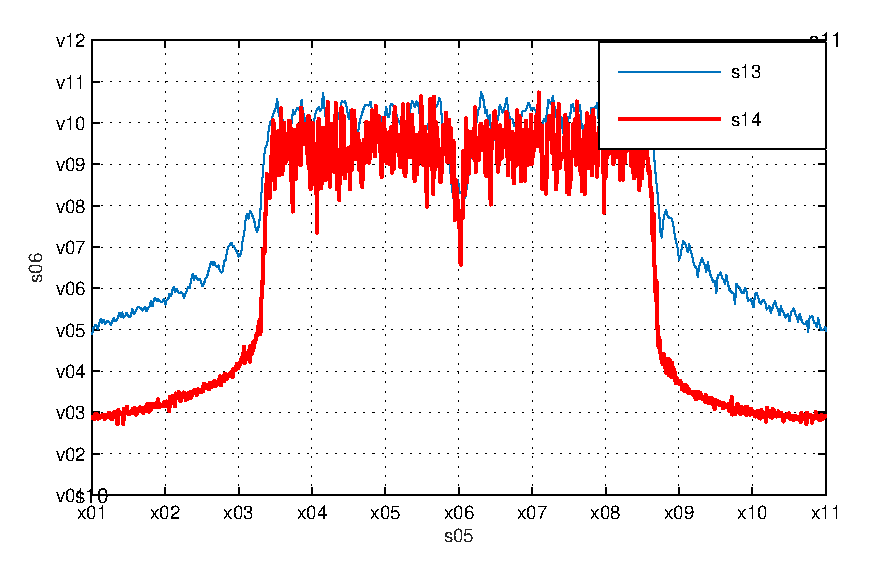
\includegraphics{OFDMvsFBMC.eps}}%
%\end{psfrags}%
%
% End OFDMvsFBMC.tex
\end{document}
% See http://www.mathworks.de/matlabcentral/fileexchange/loadFile.do?objectId=4638
% for recent versions of laprint.m.
%
% created by:           LaPrint version 3.16 (13.9.2004)
% created on:           28-Apr-2015 10:28:34
% eps bounding box:     16 cm x 12 cm
% comment:              
%
%\begin{psfrags}%
%\psfragscanon%
%
% text strings:
\psfrag{s05}[t][t]{\fontsize{9}{13.5}\fontseries{m}\mathversion{normal}\fontshape{n}\selectfont \color[rgb]{0.15,0.15,0.15}\setlength{\tabcolsep}{0pt}\begin{tabular}{c}f [MHz]\end{tabular}}%
\psfrag{s06}[b][b]{\fontsize{9}{13.5}\fontseries{m}\mathversion{normal}\fontshape{n}\selectfont \color[rgb]{0.15,0.15,0.15}\setlength{\tabcolsep}{0pt}\begin{tabular}{c}Normalized PSD [dB/Hz]\end{tabular}}%
\psfrag{s10}[][]{\fontsize{10}{15}\fontseries{m}\mathversion{normal}\fontshape{n}\selectfont \color[rgb]{0,0,0}\setlength{\tabcolsep}{0pt}\begin{tabular}{c} \end{tabular}}%
\psfrag{s11}[][]{\fontsize{10}{15}\fontseries{m}\mathversion{normal}\fontshape{n}\selectfont \color[rgb]{0,0,0}\setlength{\tabcolsep}{0pt}\begin{tabular}{c} \end{tabular}}%
\psfrag{s12}[l][l]{\fontsize{9}{13.5}\fontseries{m}\mathversion{normal}\fontshape{n}\selectfont \color[rgb]{0,0,0}FBMC}%
\psfrag{s13}[l][l]{\fontsize{9}{13.5}\fontseries{m}\mathversion{normal}\fontshape{n}\selectfont \color[rgb]{0,0,0}OFDM}%
\psfrag{s14}[l][l]{\fontsize{9}{13.5}\fontseries{m}\mathversion{normal}\fontshape{n}\selectfont \color[rgb]{0,0,0}FBMC}%
%
% axes font properties:
\fontsize{9}{13.5}\fontseries{m}\mathversion{normal}%
\fontshape{n}\selectfont%
%
% xticklabels:
\psfrag{x01}[t][t]{-2.5}%
\psfrag{x02}[t][t]{-2}%
\psfrag{x03}[t][t]{-1.5}%
\psfrag{x04}[t][t]{-1}%
\psfrag{x05}[t][t]{-0.5}%
\psfrag{x06}[t][t]{0}%
\psfrag{x07}[t][t]{0.5}%
\psfrag{x08}[t][t]{1}%
\psfrag{x09}[t][t]{1.5}%
\psfrag{x10}[t][t]{2}%
\psfrag{x11}[t][t]{2.5}%
%
% yticklabels:
\psfrag{v01}[r][r]{-70}%
\psfrag{v02}[r][r]{-65}%
\psfrag{v03}[r][r]{-60}%
\psfrag{v04}[r][r]{-55}%
\psfrag{v05}[r][r]{-50}%
\psfrag{v06}[r][r]{-45}%
\psfrag{v07}[r][r]{-40}%
\psfrag{v08}[r][r]{-35}%
\psfrag{v09}[r][r]{-30}%
\psfrag{v10}[r][r]{-25}%
\psfrag{v11}[r][r]{-20}%
\psfrag{v12}[r][r]{-15}%
%
% Figure:
%\resizebox{8cm}{!}{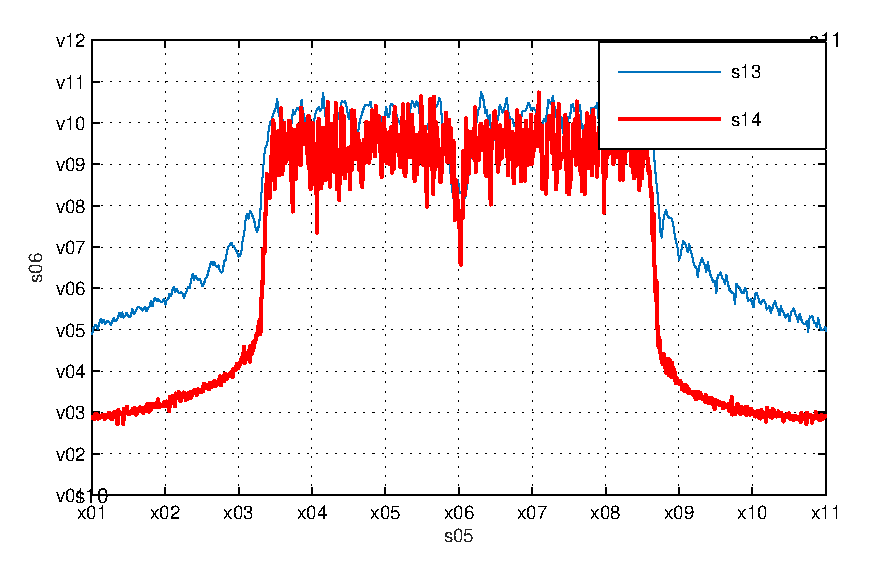
\includegraphics{OFDMvsFBMC.eps}}%
%\end{psfrags}%
%
% End OFDMvsFBMC.tex
\end{document}
% See http://www.mathworks.de/matlabcentral/fileexchange/loadFile.do?objectId=4638
% for recent versions of laprint.m.
%
% created by:           LaPrint version 3.16 (13.9.2004)
% created on:           28-Apr-2015 10:28:34
% eps bounding box:     16 cm x 12 cm
% comment:              
%
%\begin{psfrags}%
%\psfragscanon%
%
% text strings:
\psfrag{s05}[t][t]{\fontsize{9}{13.5}\fontseries{m}\mathversion{normal}\fontshape{n}\selectfont \color[rgb]{0.15,0.15,0.15}\setlength{\tabcolsep}{0pt}\begin{tabular}{c}f [MHz]\end{tabular}}%
\psfrag{s06}[b][b]{\fontsize{9}{13.5}\fontseries{m}\mathversion{normal}\fontshape{n}\selectfont \color[rgb]{0.15,0.15,0.15}\setlength{\tabcolsep}{0pt}\begin{tabular}{c}Normalized PSD [dB/Hz]\end{tabular}}%
\psfrag{s10}[][]{\fontsize{10}{15}\fontseries{m}\mathversion{normal}\fontshape{n}\selectfont \color[rgb]{0,0,0}\setlength{\tabcolsep}{0pt}\begin{tabular}{c} \end{tabular}}%
\psfrag{s11}[][]{\fontsize{10}{15}\fontseries{m}\mathversion{normal}\fontshape{n}\selectfont \color[rgb]{0,0,0}\setlength{\tabcolsep}{0pt}\begin{tabular}{c} \end{tabular}}%
\psfrag{s12}[l][l]{\fontsize{9}{13.5}\fontseries{m}\mathversion{normal}\fontshape{n}\selectfont \color[rgb]{0,0,0}FBMC}%
\psfrag{s13}[l][l]{\fontsize{9}{13.5}\fontseries{m}\mathversion{normal}\fontshape{n}\selectfont \color[rgb]{0,0,0}OFDM}%
\psfrag{s14}[l][l]{\fontsize{9}{13.5}\fontseries{m}\mathversion{normal}\fontshape{n}\selectfont \color[rgb]{0,0,0}FBMC}%
%
% axes font properties:
\fontsize{9}{13.5}\fontseries{m}\mathversion{normal}%
\fontshape{n}\selectfont%
%
% xticklabels:
\psfrag{x01}[t][t]{-2.5}%
\psfrag{x02}[t][t]{-2}%
\psfrag{x03}[t][t]{-1.5}%
\psfrag{x04}[t][t]{-1}%
\psfrag{x05}[t][t]{-0.5}%
\psfrag{x06}[t][t]{0}%
\psfrag{x07}[t][t]{0.5}%
\psfrag{x08}[t][t]{1}%
\psfrag{x09}[t][t]{1.5}%
\psfrag{x10}[t][t]{2}%
\psfrag{x11}[t][t]{2.5}%
%
% yticklabels:
\psfrag{v01}[r][r]{-70}%
\psfrag{v02}[r][r]{-65}%
\psfrag{v03}[r][r]{-60}%
\psfrag{v04}[r][r]{-55}%
\psfrag{v05}[r][r]{-50}%
\psfrag{v06}[r][r]{-45}%
\psfrag{v07}[r][r]{-40}%
\psfrag{v08}[r][r]{-35}%
\psfrag{v09}[r][r]{-30}%
\psfrag{v10}[r][r]{-25}%
\psfrag{v11}[r][r]{-20}%
\psfrag{v12}[r][r]{-15}%
%
% Figure:
%\resizebox{8cm}{!}{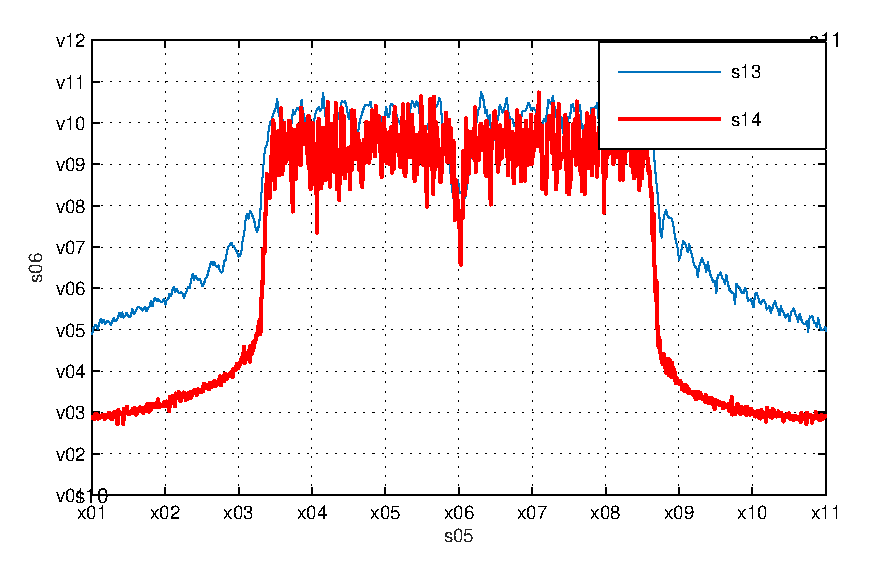
\includegraphics{OFDMvsFBMC.eps}}%
%\end{psfrags}%
%
% End OFDMvsFBMC.tex
\end{document}
% See http://www.mathworks.de/matlabcentral/fileexchange/loadFile.do?objectId=4638
% for recent versions of laprint.m.
%
% created by:           LaPrint version 3.16 (13.9.2004)
% created on:           28-Apr-2015 10:28:34
% eps bounding box:     16 cm x 12 cm
% comment:              
%
%\begin{psfrags}%
%\psfragscanon%
%
% text strings:
\psfrag{s05}[t][t]{\fontsize{9}{13.5}\fontseries{m}\mathversion{normal}\fontshape{n}\selectfont \color[rgb]{0.15,0.15,0.15}\setlength{\tabcolsep}{0pt}\begin{tabular}{c}f [MHz]\end{tabular}}%
\psfrag{s06}[b][b]{\fontsize{9}{13.5}\fontseries{m}\mathversion{normal}\fontshape{n}\selectfont \color[rgb]{0.15,0.15,0.15}\setlength{\tabcolsep}{0pt}\begin{tabular}{c}Normalized PSD [dB/Hz]\end{tabular}}%
\psfrag{s10}[][]{\fontsize{10}{15}\fontseries{m}\mathversion{normal}\fontshape{n}\selectfont \color[rgb]{0,0,0}\setlength{\tabcolsep}{0pt}\begin{tabular}{c} \end{tabular}}%
\psfrag{s11}[][]{\fontsize{10}{15}\fontseries{m}\mathversion{normal}\fontshape{n}\selectfont \color[rgb]{0,0,0}\setlength{\tabcolsep}{0pt}\begin{tabular}{c} \end{tabular}}%
\psfrag{s12}[l][l]{\fontsize{9}{13.5}\fontseries{m}\mathversion{normal}\fontshape{n}\selectfont \color[rgb]{0,0,0}FBMC}%
\psfrag{s13}[l][l]{\fontsize{9}{13.5}\fontseries{m}\mathversion{normal}\fontshape{n}\selectfont \color[rgb]{0,0,0}OFDM}%
\psfrag{s14}[l][l]{\fontsize{9}{13.5}\fontseries{m}\mathversion{normal}\fontshape{n}\selectfont \color[rgb]{0,0,0}FBMC}%
%
% axes font properties:
\fontsize{9}{13.5}\fontseries{m}\mathversion{normal}%
\fontshape{n}\selectfont%
%
% xticklabels:
\psfrag{x01}[t][t]{-2.5}%
\psfrag{x02}[t][t]{-2}%
\psfrag{x03}[t][t]{-1.5}%
\psfrag{x04}[t][t]{-1}%
\psfrag{x05}[t][t]{-0.5}%
\psfrag{x06}[t][t]{0}%
\psfrag{x07}[t][t]{0.5}%
\psfrag{x08}[t][t]{1}%
\psfrag{x09}[t][t]{1.5}%
\psfrag{x10}[t][t]{2}%
\psfrag{x11}[t][t]{2.5}%
%
% yticklabels:
\psfrag{v01}[r][r]{-70}%
\psfrag{v02}[r][r]{-65}%
\psfrag{v03}[r][r]{-60}%
\psfrag{v04}[r][r]{-55}%
\psfrag{v05}[r][r]{-50}%
\psfrag{v06}[r][r]{-45}%
\psfrag{v07}[r][r]{-40}%
\psfrag{v08}[r][r]{-35}%
\psfrag{v09}[r][r]{-30}%
\psfrag{v10}[r][r]{-25}%
\psfrag{v11}[r][r]{-20}%
\psfrag{v12}[r][r]{-15}%
%
% Figure:
%\resizebox{8cm}{!}{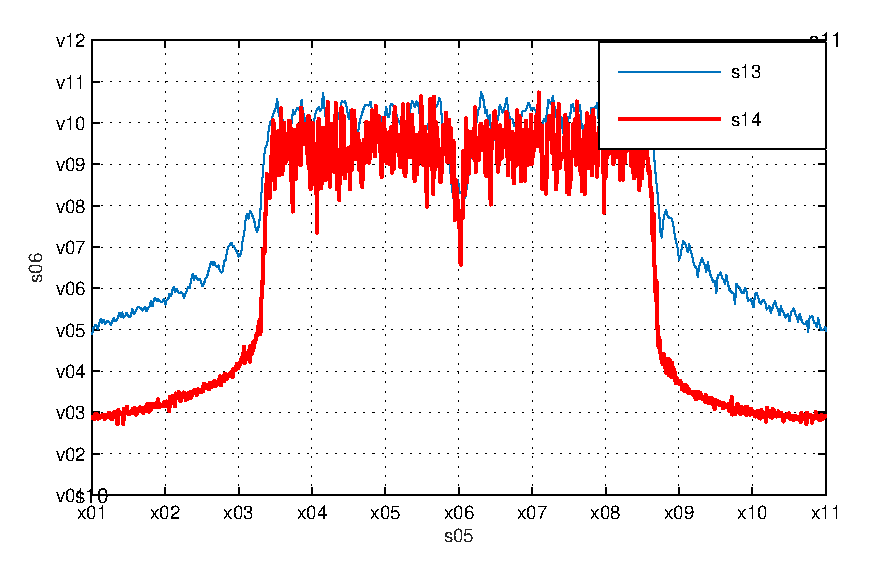
\includegraphics{OFDMvsFBMC.eps}}%
%\end{psfrags}%
%
% End OFDMvsFBMC.tex
